\documentclass[10pt]{beamer}
\usetheme[left]{AAUsidebar}

% If you want to change the colors of the various elements in the theme, edit and uncomment the following lines
% Change the bar and sidebar colors:
%\setbeamercolor{AAUsidebar}{fg=red!20,bg=red}
%\setbeamercolor{sidebar}{bg=red!20}
% Change the color of the structural elements:
%\setbeamercolor{structure}{fg=red}
% Change the frame title text color:
%\setbeamercolor{frametitle}{fg=blue}
% Change the normal text color background:
%\setbeamercolor{normal text}{bg=gray!10}
% ... and you can of course change a lot more - see the beamer user manual.

\usepackage[utf8]{inputenc}
\usepackage[english]{babel}
\usepackage[T1]{fontenc}
% Or whatever. Note that the encoding and the font should match. If T1
% does not look nice, try deleting the line with the fontenc.
\usepackage{helvet}

% colored hyperlinks
\newcommand{\chref}[2]{%
  \href{#1}{{\usebeamercolor[bg]{AAUsidebar}#2}}%
}

\title[Managing Global Software Projects]% optional, use only with long paper titles
{Managing Global Software Projects}

%\subtitle{v.\ 1.4.0}  % could also be a conference name

\date{%\today
	}

\author[Leonel Muñoz Cedano] % optional, use only with lots of authors
{
  Leonel Muñoz Cedano\\
  \href{mailto:leoneling@gmail.com}{{\tt leoneling@gmail.com}}
}
% - Give the names in the same order as they appear in the paper.
% - Use the \inst{?} command only if the authors have different
%   affiliation. See the beamer manual for an example

\institute[
%  {\includegraphics[scale=0.2]{aau_segl}}\\ %insert a company, department or university logo
  Universidad Distrital Francisco José de Caldas\\
  Maestría en CIC\\
  Tendencias en IS\\
  Bogotá DC, 14 de Mayo
] % optional - is placed in the bottom of the sidebar on every slide
{% is placed on the title page
  Universidad Distrital Francisco José de Caldas\\
  Maestría en Ciencias de la información y las comunicaciones\\
  Tendencias en Ingeniería de Software\\
  Bogotá DC, 14 de Mayo 2016
  
  %there must be an empty line above this line - otherwise some unwanted space is added between the university and the country (I do not know why;( )
}


% specify a logo on the titlepage (you can specify additional logos an include them in 
% institute command below
\pgfdeclareimage[height=3.5cm]{titlepagelogo}{AAUgraphics/escudoudblancoynegro} % placed on the title page
%\pgfdeclareimage[height=1.5cm]{titlepagelogo2}{graphics/aau_logo_new} % placed on the title page
\titlegraphic{% is placed on the bottom of the title page
  \pgfuseimage{titlepagelogo}
%  \hspace{1cm}\pgfuseimage{titlepagelogo2}
}


\begin{document}
% the titlepage
{\aauwavesbg%
\begin{frame}[plain,noframenumbering] % the plain option removes the sidebar and header from the title page
  \titlepage
\end{frame}}
%%%%%%%%%%%%%%%%

% TOC
\begin{frame}{Agenda}{}
\tableofcontents
\end{frame}

%%%%%%%%%%%%%%%%%%%%%%%%%%%%%%%%%%%%%%%%%%%%%%%%%%%%%%%%%%%%%%%

\section{Introduction}
% motivation for creating this theme
\begin{frame}{Introduction}{Distributed projects}
  %The present beamer theme called the \alert{AAU Sidebar Beamer Theme} is an attempt to
  \begin{figure}[H] 
  	%\centering
  	\begin{flushleft}
  		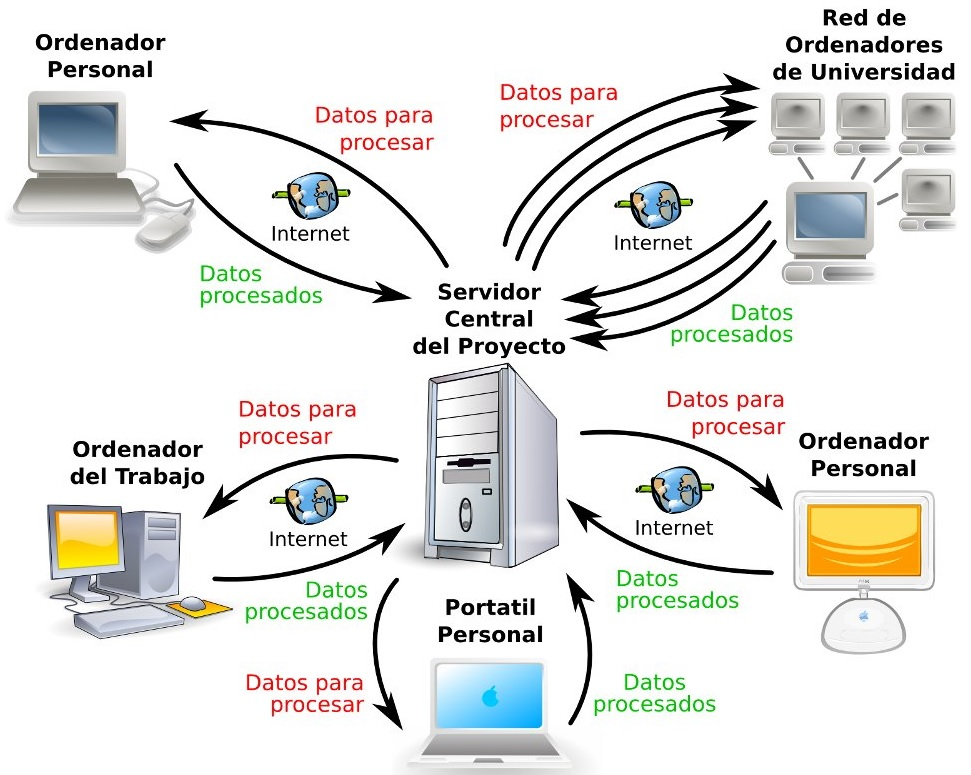
\includegraphics[width=0.85\textwidth]{./AAUgraphics/ProyectosDistribuidos.jpg}
  		\caption{Distributed projects}
  		\label{DCP}
  	\end{flushleft}
  \end{figure}
\end{frame}

%%%%%%%%%%%%%%%%%%%%%%%%%%%%%%%%%%%%%%%%%%%%%%%%%%%%%%%%%%%%%%%

\section{Foundations}
% general installation instructions
\begin{frame}{Foundations}{Reasons for outsourcing and offshoring}  
	\begin{figure}[H] 
		%\centering
		\begin{flushleft}
			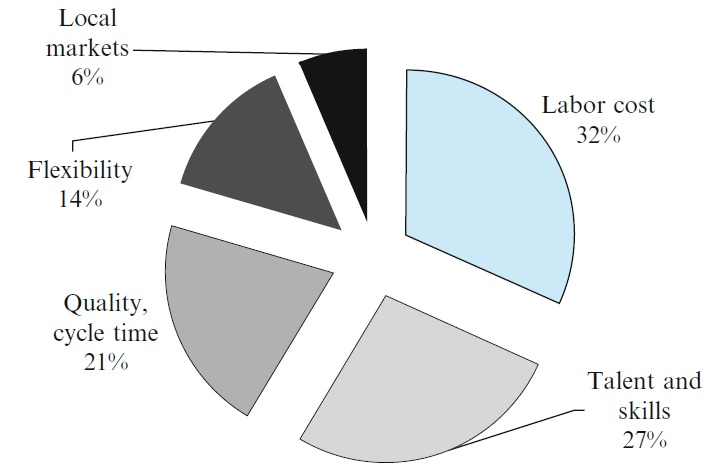
\includegraphics[width=0.90\textwidth]{./AAUgraphics/fundamentos.jpg}
			\caption{Reasons for outsourcing and offshoring}
			\label{DCP}
		\end{flushleft}
	\end{figure}
\end{frame}

%%%%%%%%%%%%%%%%%%%%%%%%%%%%%%%%%%%%%%%%%%%%%%%%%%%%%%%%%%%%%%%
\section{Benefits and Challenges}
\begin{frame}{Benefits and Challenges}{}
	The challenges in global software can be summarized as follows:
	\begin{itemize}
		\item<1-> Lack of strategy and shared values.
		\item<1-> Insufficient communication.
		\item<1-> Dispersed work organization.
		\item<1-> Inadequate global management.		
		\item<1-> Isolated learning.
		\item<1-> Insufficient contract management.
		\item<1-> Unknown legal environment.
		\item<1-> High employee turnover rate.
	\end{itemize}
\end{frame}

%%
%%%%%%%%%%%%%%%%%%%%%%%%%%%%%%%%%%%%%%%%%%%%%%%%%%%%%%%%%%%%%%%

\section{Global Software Development}
% general installation instructions
\begin{frame}{Global Software Development}{Model CMMI - Capability Maturity Model Integration}  
	\begin{figure}[H] 
		%\centering
		\begin{flushleft}
			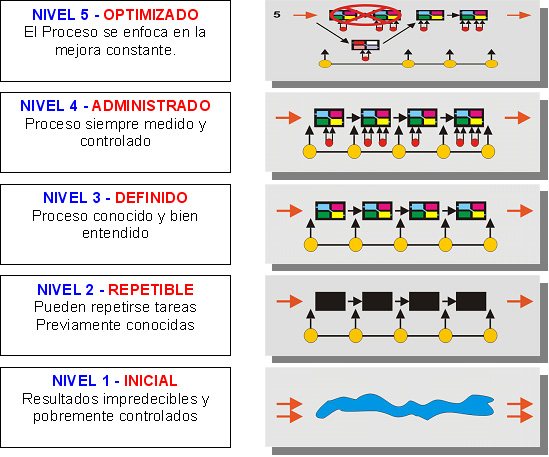
\includegraphics[width=0.80\textwidth]{./AAUgraphics/cmmi.jpg}
			\caption{Model CMMI}
			\label{DCP}
		\end{flushleft}
	\end{figure}
\end{frame}


%%
%%%%%%%%%%%%%%%%%%%%%%%%%%%%%%%%%%%%%%%%%%%%%%%%%%%%%%%%%%%%%%%
\section{Work Organization}
% general installation instructions
\begin{frame}{Work Organization}{Team work}  
	\begin{figure}[H] 
		%\centering
		\begin{flushleft}
			
\includegraphics[width=0.80\textwidth]{./AAUgraphics/Organization-Work.jpg}
			\caption{Team work}
			\label{DCP}
		\end{flushleft}
	\end{figure}
\end{frame}

%% 
%%%%%%%%%%%%%%%%%%%%%%%%%%%%%%%%%%%%%%%%%%%%%%%%%%%%%%%%%%%%%%%
\section{Risk Management}
% general installation instructions
\begin{frame}{Risk Management}{Risk Management in Global Software Projects}  
	\begin{figure}[H] 
		%\centering
		\begin{flushleft}
			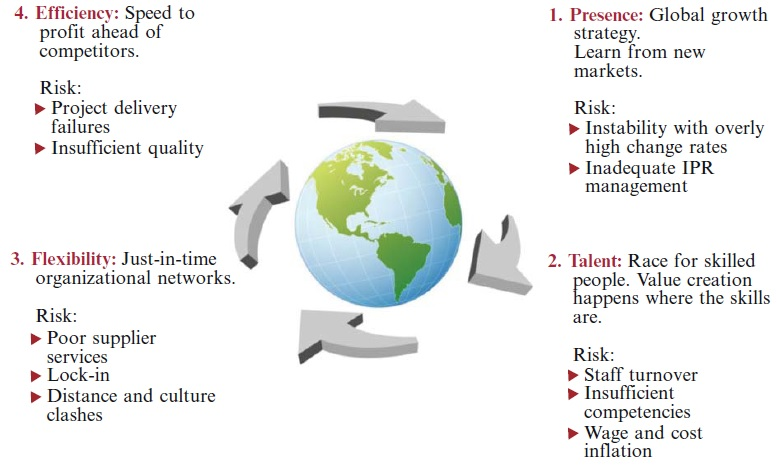
\includegraphics[width=0.95\textwidth]{./AAUgraphics/risk.jpg}
			\caption{The top 10 global software risks and their underlying drivers}
			\label{DCP}
		\end{flushleft}
	\end{figure}
\end{frame}

%%%%%%%%%%%%%%%%%%%%%%%%%%%%%%%%%%%%%%%%%%%%%%%%%%%%%%%%%%%%%%%
\section{Feedback}
\subsection{Questions, Comments and Suggestions}
% help me iron out the bugs or give me some comment and suggestions
\begin{frame}{Feedback}{Bugs, Comments and Suggestions}
  \begin{itemize}
    \item<1-> Any Question, Comment or Suggestion.
  \end{itemize}
\end{frame}
%%%%%%%%%%%%%%%%

\subsection{Contact Information}
% contact information
\begin{frame}{Feedback}{Contact Information}
In case you have comments, suggestions or questions, please do not hesitate to contact me. You can find my contact details below.
  \begin{center}
    \insertauthor\\
  \end{center}
\end{frame}
%%%%%%%%%%%%%%%%%%%%%%%%%%%%%%%%%%%%%%%%%%%%%%%%%%%%%%%%%%%%%%%%

\section{Bibliography}
\begin{frame}{Bibliography}{}

	\begin{itemize}
		\item<1->Günther Ruhe and Claes Wohlin, Software Project 	Management in a Changing World, Springer Heidelberg New York Dordrecht London 2014.
		\item<1->Ebert C (2012) Global software and IT: a guide to distributed development, projects, and outsourcing. Wiley, New York. 
		\item<1->Forrester’s Forrsights Services Survey Q2 (2012) http://www.forrester.com/Forrsights+Services	+Survey+Q2+2012/-/E-SUS1391. Accessed on 15 Aug 2013.
		\item<1->Carmel E, Espinosa JA (2012) I’m working while they’re sleeping: time zone separation challenges and solutions. Nedder Stream Press, New York.
	\end{itemize}
\end{frame}


%%%%%%%%%%%%%%%%%%%%%%%%%%%%%%%%%%%%%%%%%%%%%%%%%%%%%%%%%%%%%%%%


{\aauwavesbg
\begin{frame}[plain,noframenumbering]
  \finalpage{Thank you!}
\end{frame}}
%%%%%%%%%%%%%%%%

\end{document}
